\chapter{Описание выпуклых многогранников}
\label{cha:1}

\epigraph{
	\textit{Как многогранен этот мир и многолик!}

    \textit{А мы в нем только временные странники...}

    \textit{Мы - путники, пришедшие на миг...}

    \textit{Мы - отражающие вечность многогранники!}}
{-- Аллиса Невдомек}


Барицентрическая комбинация точек с неотрицательными коэффициентами называется \textit{выпуклой}.

Совокупность выпуклых комбинаций некоторой системы точек M называется их \textit{выпуклой оболочкой} $conv M$. 

Выпуклая комбинация $m + 1$ точки, находящихся в общем положении, называется \textit{$m$-мерным симплексом}.

Например, одномерный симплекс – это отрезок, двумерный симплекс – это треугольник, трехмерный симплекс – тетраэдр.

\begin{propose}[]\label{cha:1/propose:1}
	Выпуклая комбинация точек не зависит от выбора внешней точки. Выпуклая комбинация точек n-мерного аффинного пространства совпадает с выпуклой комбинацией не более, чем $n + 1$ точек из них.
\end{propose}
\begin{Proof}
	Рассмотрим выпуклую комбинацию точек $A_0, \dots, A_m$, где $m > n$:
	$$O + \underset{j=0}{\overset{m}{\sum}}\lambda_j \overline{OA_j}, \; \lambda_j > 0, \; \underset{j=0}{\overset{m}{\sum}}\lambda_j = 1$$
	Так как векторы $A_0A_1, \dots, A_0A_m$ линейно зависимы, то существует нетривиальная линейная комбинация $\displaystyle c_1 \overline{A_0 A_1} + \dots + c_m \overline{A_0 A_m} = 0$. Полагая $A_0A_j = OA_j − OA_0$, получим равенство:
	$$\alpha_0 \overline{O A_0} + \dots + \alpha_m \overline{O A_m} = 0, \; \alpha_j = \begin{cases}
		c_j, \text{ если } j=\ton m \\
		-c_1 - \dots - c_m, \text{ если } j = 0
	\end{cases}$$
	Тогда $\underset{j=0}{\overset{m}{\sum}}\alpha_j = 0$.  Без ограничения общности можно считать, что некоторое $\alpha_j > 0$. Пусть $\theta = \underset{j: \alpha_j > 0}{\min}\frac{\lambda_j}{\alpha_j}$. В этом случае $\theta > 0$, причем:
	$$O + \underset{j=0}{\overset{m}{\sum}}\lambda_j \overline{O A_j} = O + \underset{j=0}{\overset{m}{\sum}}(\lambda_j - \theta \alpha_j) \overline{OA_j}$$
	Для положительных $\alpha_j$ имеем $\displaystyle \lambda_j - \theta \alpha_j = \alpha_j \left( \frac{\lambda_j}{\alpha_j} - \theta \right)$. Для отрицательных $\alpha_j$ это неравенство тем более имеет место. При этом хотя бы для одного $j$ справедливо равенство $\lambda_j − \theta \alpha_j = 0$. Кроме того:
	$$\underset{j=0}{\overset{m}{\sum}}(\lambda_j - \theta \alpha_j) = \underset{j=0}{\overset{m}{\sum}}\lambda_j - \theta \underset{j=0}{\overset{m}{\sum}}\alpha_j = 1$$
\end{Proof}

\begin{definition}\label{cha:1/def:1}
	Множество точек \blue{выпукло}, если оно вместе с любыми двумя своими точками содержит соединяющиий их отрезок.
\end{definition}

\begin{definition}\label{cha:1/def:2}
	Наименьшее по включению выпуклое множество, содержащее данное множество точек $\{A_0, \dots, A_m\}$ называется \blue{выпуклым замыканием} и обозначается $conv\{A_0, \dots, A_m\}$.
\end{definition}

\begin{theorem}[]\label{cha:1/the:1}
	Выпуклое замыкание $M = conv\{A_0, \dots, A_m\}$ состоит из всех точек следующего вида:
	$$A = O + \underset{j=0}{\overset{m}{\sum}}\alpha_j \overline{O A_j}, \; \underset{j=0}{\overset{m}{\sum}}\alpha_j = 1, \; \alpha_j \ge 0\eqno(1)$$
\end{theorem}
\begin{Proof}
	Пусть $A$ из (1) и
	$$B = O + \underset{j=0}{\overset{m}{\sum}}\beta_j \overline{O A_j} \in M, \; \underset{j=0}{\overset{m}{\sum}}\beta_j = 1, \; \beta_j \ge 0$$
	Пусть $0 \le \alpha, \beta \le 1$ и $\alpha + \beta = 1$. Тогда:
	$$\begin{gathered}
		O + \alpha \overline{OA} + \beta \overline{OB} = O + \alpha \underset{j=0}{\overset{m}{\sum}}\alpha_j \overline{OA_j} + \beta \left( \underset{j=0}{\overset{m}{\sum}}\beta_j \overline{OA_j} \right) = \\
		= O + \underset{j=0}{\overset{m}{\sum}} (\alpha \alpha_j + \beta \beta_j) \overline{OA_j} \in M \\
		\text{ т.к. } \underset{j=0}{\overset{m}{\sum}} (\alpha \alpha_j + \beta \beta_j) = \alpha \underset{j=0}{\overset{m}{\sum}}\alpha_j + \beta \underset{j=0}{\overset{m}{\sum}}\beta_j = \alpha + \beta = 1
	\end{gathered}$$
	Следовательно, $M$ – выпуклое множество. Кроме того, $\{A_0, \dots, A_m\} \in M$.

	Покажем обратное включение. Пусть $N$ — выпуклое множество, содержащее $A_0, \dots, A_m$. Индукцией по $m$ установим, что точка $A$ из (1) в лежит в $N$.

	Если $m = 0$, то $conv A_0 = A_0 \in N$.

	Пусть $m = 1$. Тогда при $\alpha_0, \alpha_1 \ge 0$ и $\alpha_0 + \alpha_1 = 1$, откуда получаем:
	$$A = O + \alpha_0 \overline{OA_0} + \alpha_1 \overline{OA_1} \in \left[ A_0, A_1 \right] \subseteq N\eqno(2)$$
	Пусть для случая $m − 1$ утверждение доказано и $m \ge 2$. Возьмем точку $A$ из (1). Можно считать, например, что $1 > \alpha_m > 0$. Тогда: 
	$$\begin{gathered}
		B = O + \underset{j=0}{\overset{m-1}{\sum}}\frac{\alpha_j}{1-\alpha_m}\overline{OA_j} \in N \text{ по индукции}, \\
		\text{т.к. } \underset{j=0}{\overset{m-1}{\sum}}\frac{\alpha_j}{1-\alpha_m} = \frac{1-\alpha_m}{1-\alpha_m} = 1
	\end{gathered}$$
	При этом как и в (2):
	$$A = O + (1-\alpha_m)\underset{j=1}{\overset{m-1}{\sum}}\frac{\alpha_j}{1-\alpha_m}\overline{OA_j} + \alpha_m \overline{OA_m} \in \left[ B, A_m \right] \subseteq N$$
	Следовательно, $M \subseteq N$.
\end{Proof}

\begin{definition}\label{cha:1/def:3}
	Выпуклое замыкание конечного числа точек называется \blue{выпуклым многогранником}.
\end{definition}

\begin{theorem}[]\label{cha:1/the:2}
	В n-мерном евклидовом пространстве выпуклое множество размерности n обладает внутренними точками.
\end{theorem}
\begin{Proof}
	Выпуклое множество размерности n содержит $n+1$ точку в общем положении и, следовательно, в нем лежит порожденный ими n-мерный симплекс, обладающий внутренними точками.
\end{Proof}

\begin{definition}\label{cha:1/def:4}
	Совокупность всех внутренних точек множества $M \subseteq S$ называется его \textit{внутренностью} и обозначается $int M$, а совокупность граничных точек — его \textit{границей} и обозначается $bd M$.
\end{definition}

\begin{definition}\label{cha:1/def:5}
	Множество M, полученное присоединением к M его граничных точек, называется \blue{замыканием} M. Таким образом, $\overline{M} = M \cup bd M$. Множество M замкнуто, если $M = \overline{M}$.
\end{definition}

\begin{propose}[]\label{cha:1/propose:2}
	Внутренность выпуклого множества является выпуклым множеством.
\end{propose}
\begin{Proof}
	Пусть $A, B \in int M$ и $C \in [A, B]$. Покажем, что $C$ является внутренней точкой множества $M$. Это вытекает из элементарных геометрических соображений. Существует такое $r > 0$, что шары с центрами $A$ и $B$ радиуса $r$ лежат в $M$. 

	\begin{center}
		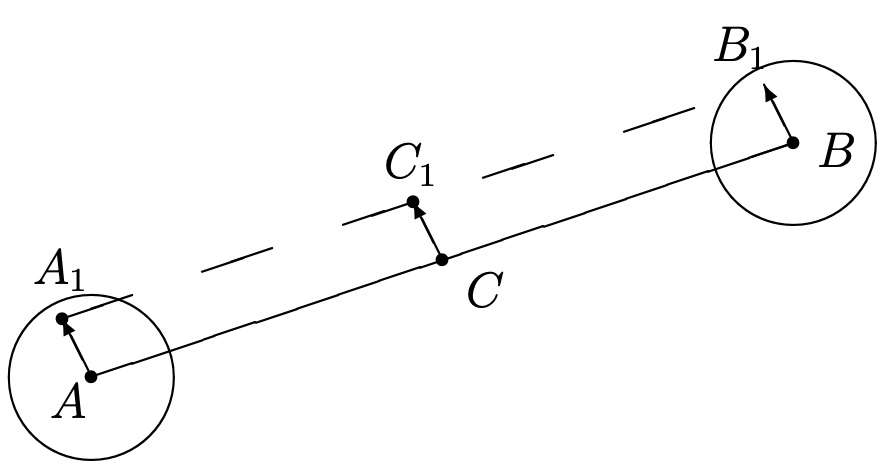
\includegraphics[width = \textwidth]{1_1}
	\end{center}

	Пусть $C_1$ – любая точка, удаленная от $C$ на расстояние $\le r$. Тогда в упомянутых шарах можно выбрать, соответственно, точки $A_1, B_1$ так, чтобы выполнялись равенства $\overline{AA_1} = \overline{CC_1} = \overline{BB_1}$. По условию $A_1, B_1 \in M$ и в силу выпуклости множества $M$ справедливо включение $[A_1, B_1] \in M$. Но $C_1 \in [A_1, B_1]$ и потому $C_1 \in M$. Таким образом, окрестность точки $C$ радиуса $r$ лежит в $M$, т. е. $C$ – внутренняя точка. Значит, $[A, B] \subseteq int M$ и $int M$ – выпуклое множество.

\end{Proof}

\begin{propose}[]\label{cha:1/clair:2}
	Замыкание $\overline{M}$ выпуклого множества $M$ является выпуклым множеством.
\end{propose}
\begin{Proof}
	Пусть $A, B \in M$ и:
	$$C = O + \lambda \overline{OA} + \mu \overline{OB} \in [A, B], \; \lambda, \mu \ge 0, \; \lambda + \mu = 1$$
	Из очевидных соображений для любого $\varepsilon > 0$ существует такое $\delta > 0$, что как только точки $A_1$ и $B_1$ находятся в $\delta$-окрестности, соответственно, точек $A$ и $B$, то точка $\displaystyle C_1 = O + \lambda \overline{OA_1} + \mu \overline{OB_1} \in [A_1, B_1]$ лежит в $\varepsilon$-окрестности точки $C$. По условию точки $A_1$, $B_1$ можно выбрать лежащими в $M$ и в силу выпуклости M точка $C_1$ лежит в M . Итак, в любой окрестности точки C лежат точки из M , поэтому C либо внутренняя, либо граничная точка M. В обоих случаях $C \in \overline{M}$. Нами доказано, что $[A,B] \subseteq \overline{M}$ и, следовательно, $\overline{M}$ – выпуклое множество.

\end{Proof}

\begin{lemma}\label{cha:1/lemma:1}
	Выпуклое замыкание объединения двух выпуклых множеств M и N совпадает с объединением отрезков, соединяющих пары точек этих множеств:
	$$[M \cup N] = \cup [A, B], \; A \in M, B \in N$$
\end{lemma}
\begin{Proof}
	По теореме \ref{cha:1/the:1} точка $C \in [M \cup N ]$ обладает представлением следующего вида:
	$$\begin{gathered}
		C = O + \underset{j=1}{\overset{p}{\sum}}\lambda_j \overline{OA_j} + \underset{j=1}{\overset{q}{\sum}}\mu_j \overline{O B_j}, \; \lambda_j, \mu_j \ge 0 \\
		\underset{j=1}{\overset{p}{\sum}}\lambda_j + \underset{j=1}{\overset{q}{\sum}}\mu_j = 1, \; A_1, \dots, A_p \in M, \; B_1, \dots, B_q \in N
	\end{gathered}$$
	Положим:
	$$\lambda = \underset{j=1}{\overset{p}{\sum}}\lambda_j \ge 0, \; \mu = \underset{j=1}{\overset{q}{\sum}}\mu_j \ge 0$$
	Тогда $\lambda + \mu = 1$ и:
	$$A = O + \underset{j=1}{\overset{p}{\sum}}\frac{\lambda_j}{\lambda} \overline{OA_j}, \; B = O + \underset{j=1}{\overset{q}{\sum}}\frac{\mu_j}{\mu} \overline{OB_j}$$
	Следовательно, $C \in [A, B]$, $A \in M$, $B \in N$, поскольку $\displaystyle C = O + \lambda \overline{OA} + \mu \overline{OB}$.
\end{Proof}

\begin{definition}\label{cha:1/def:6}
	Точка выпуклого множества называется \blue{угловой}, если она не принадлежит внутренности отрезка, целиком лежащего в этом множестве.
\end{definition}

\begin{conseq}[]\label{cha:1/conseq:1}
	Пусть M выпуклое множество и точка $A \not \in M$. Тогда A является угловой точкой выпуклого замыкания $[M \cup A]$.
\end{conseq}
\begin{Proof}
	По лемме \ref{cha:1/lemma:1} концы отрезка $[P, Q] \subseteq [M \cup A]$ принадлежат, соответственно, отрезкам: $Q \in [A,B]$, $B \in M$, и $P \in [A, C]$, $C \in M$. 

	\begin{center}
		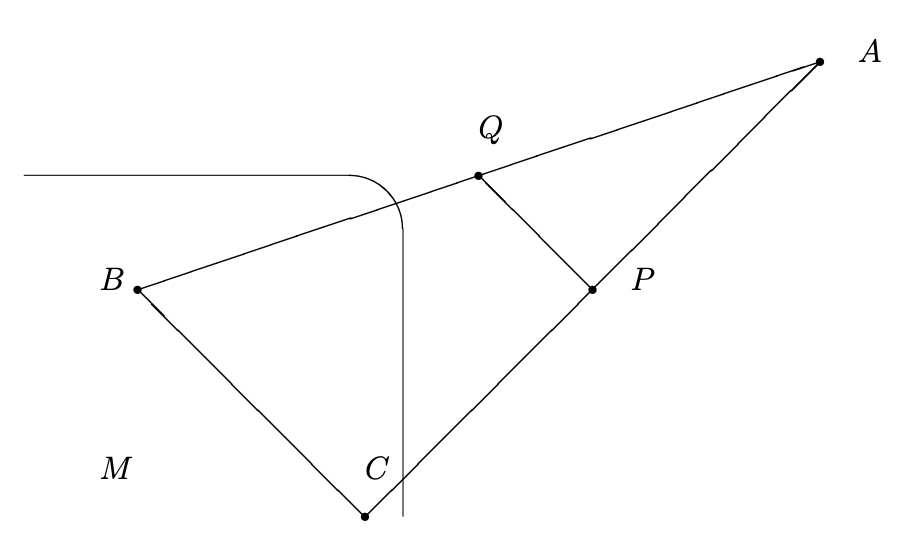
\includegraphics[width = \textwidth]{1_2}
	\end{center}

	Из треугольника $ABC$ видно, что при любых возможных положениях точек $P, Q$ точка A не принадлежит внутренности отрезка $[P,Q]$. Это рассуждение включает в себя и предельный случай $B = C$.
\end{Proof}

\begin{theorem}[]\label{cha:1/the:3}
	Выпуклый многогранник совпадает с выпуклым замыканием своих угловых точек.
\end{theorem}
\begin{Proof}
	Выбросим последовательно те порождающие точки выпуклого многогранника $M$ , которые принадлежат выпуклому замыканию остальных точек. Оставшиеся точки порождают многогранник $M$, причем по следствию \ref{cha:1/conseq:1} каждая из них является угловой.
\end{Proof}

\begin{theorem}[]\label{cha:1/the:4}
	Выпуклый многогранник является замкнутым множеством.
\end{theorem}
\begin{Proof}
	Из предложения \ref{cha:1/propose:1} вытекает, что каждая точка выпуклого многогранника M принадлежит симплексу некоторой размерности, целиком лежащему в M, и порождено некоторым множеством угловых точек, находящихся в общем положении. Таким образом, M совпадает с объединением конечного числа симплексов. Но каждый симплекс является замкнутым множеством, и поэтому M – замкнутое множество.
\end{Proof}






















